\documentclass[12pt, oneside, a4paper, chapter=TITLE,section=TITLE]{abntex2}

\usepackage{abntex2-ifrj} % pacote com customizações da classe abntex2 para uso no IFRJ-CVR

%Carregando alguns pacotes extras
\usepackage{float}
\usepackage{scalefnt}
\usepackage{supertabular,booktabs}
\usepackage{multirow}
\usepackage{graphicx}
\usepackage{tikz}
\usetikzlibrary{shapes,arrows.meta,positioning,calc,fit,backgrounds}

% Estilos reutilizados nos wireframes de baixa fidelidade
\tikzset{
  moldura/.style={draw=black!85, ultra thick, rounded corners=2pt},
  cabecalho/.style={draw=black!75, very thick, fill=black!10, minimum width=4.2cm,
    minimum height=0.7cm, align=center, font=\scriptsize\bfseries},
  categoria/.style={draw=black!65, fill=black!5, minimum width=1.2cm,
    minimum height=0.45cm, align=center, font=\scriptsize},
  cartao/.style={draw=black!70, very thick, minimum width=4.2cm, minimum height=1.15cm,
    align=left, font=\scriptsize},
  botao/.style={draw=black!80, very thick, fill=black!6, rounded corners=2pt,
    minimum width=1.5cm, minimum height=0.45cm, align=center, font=\scriptsize},
  campo/.style={draw=black!60, minimum width=4.2cm, minimum height=0.45cm,
    align=left, font=\scriptsize},
  opcao/.style={draw=black!65, very thick, minimum width=4.2cm, minimum height=0.42cm,
    align=left, font=\scriptsize},
  botaq/.style={draw=black!80, very thick, fill=black!6, rounded corners=2pt,
    minimum width=0.8cm, minimum height=0.45cm, align=center, font=\scriptsize}
}

% ---
% Informações de dados para CAPA e FOLHA DE ROSTO
% ---
\titulo{Totem de Autoatendimento para Restaurantes de Cidades Pequenas: Entrega Parcial 2}
\tipotrabalho{Relatório Técnico para Engenharia de Software}
\autor{Alunos: Gabriel Muzel e Mateus Iuri \\ Profa. Dra. Suéllen Martinelli }

\local{Capão Bonito}
\data{\today}
\programa{Tecnologia em Sistemas Inteligentes}
% Preâmbulo
\preambulo{\imprimirtipotrabalho\, desenvolvido pelos alunos Gabriel Muzel e Mateus Iuri como parte dos critérios de avaliação da disciplina ministrada pela Profa. Dra. Suéllen Martinelli. Esta entrega documenta a execução da primeira Sprint: protótipo de baixa fidelidade, diagramas de caso de uso, captura de feedback e eventos de encerramento.
}

% --------------------------------
\makeindex % compila o índice remissivo (opcional)
% --------------------------------

% --------------------------------
% Início do documento
% --------------------------------
\begin{document}

% Retira espaço extra obsoleto entre as frases.
\frenchspacing

% --------------------------------
% ELEMENTOS PRÉ-TEXTUAIS
% --------------------------------
\pretextual
% ---
\imprimircapa % Capa
\imprimirfolhaderosto % Folha de rosto
% ---

% ---
% lista de ilustrações
\pdfbookmark[0]{\listfigurename}{lof} \listoffigures*
\cleardoublepage
% ---

% ---
% lista de tabelas
\pdfbookmark[0]{\listtablename}{lot}\listoftables*
\cleardoublepage
% ---

% ---
% inserir lista de quadros
\pdfbookmark[0]{\listofquadrosname}{loq} \listofquadros*
\cleardoublepage
% ---

% ---
% inserir lista de abreviaturas e siglas (opcional)
\begin{siglas}
  \item[ABNT] Associação Brasileira de Normas Técnicas
  \item[CSV] \textit{Comma-Separated Values}
  \item[LF] Baixa Fidelidade
  \item[PO] Product Owner
  \item[SM] Scrum Master
  \item[TCLE] Termo de Consentimento Livre e Esclarecido
  \item[UC] Caso de Uso
  \item[US] História de Usuário
  \item[WIP] Work In Progress
\end{siglas}
% ---

% ---
% inserir lista de símbolos
% ---
\begin{simbolos}
  \item[$N$] Número de participantes do teste de usabilidade
\end{simbolos}
% ---

% ---
% sumario
\pdfbookmark[0]{\contentsname}{toc}
\tableofcontents*
% ---

% --------------------------------
% ELEMENTOS TEXTUAIS
\textual
% --------------------------------

\chapter{Introdução}

Esta entrega dá continuidade ao planejamento registrado na Parcial 1. O escopo considerado é a Sprint 1, cujo \textit{Sprint Backlog} continha três histórias: US01 (Visualizar Cardápio), US02 (Adicionar Item) e US03 (Personalizar Pedido). Assim, todo o protótipo, os diagramas e a coleta de feedback aqui apresentados estão limitados a essas três histórias.

\chapter{Características do Projeto}

O projeto investiga um totem de autoatendimento para restaurantes de cidades pequenas. A primeira entrega concentrou a descoberta e o planejamento de requisitos; esta segunda entrega registra a execução da Sprint 1, com prototipação de baixa fidelidade, modelagem de casos de uso, teste com participantes e os eventos de Sprint Review e Retrospectiva.

Os dados quantitativos e qualitativos da Parcial 1 foram tabulados a partir do arquivo \texttt{formulario\_andromeda.csv}, com 13 respostas anônimas. As funcionalidades mais votadas foram pagamento integrado (10), personalização (9), emissão de senha (8), fotos (5), acessibilidade (5) e fidelidade (5).

\section{Problema e Objetivo}

\textbf{Problema:} a execução da Sprint 1 precisa ser validada antes da implementação definitiva, para evitar que falhas de navegação, clareza e acessibilidade cheguem ao código.

\textbf{Objetivo geral:} validar, com baixo custo, o fluxo das US01, US02 e US03 por meio de protótipo de baixa fidelidade, diagramas de caso de uso e captura de feedback.

\begin{itemize}
    \item Apresentar as versões inicial e completa do protótipo de baixa fidelidade.
    \item Apresentar os diagramas de caso de uso nas versões inicial e digital.
    \item Coletar feedback de, no mínimo, quatro participantes sobre o protótipo.
    \item Relatar a Sprint Review e a Retrospectiva e o antes e depois do Kanban e do \textit{Product Backlog}.
\end{itemize}

\section{Metodologia Utilizada: SCRUM}

O SCRUM estrutura o trabalho em papéis, artefatos e eventos \cite{schwaber2017scrum}. Nesta entrega, o \textit{Sprint Backlog} da Sprint 1 define o escopo, a Sprint Review demonstra as funcionalidades e a Retrospectiva registra aprendizados e ajustes. A Engenharia de Requisitos complementa o processo com Histórias de Usuário e critérios de aceitação \cite{wazlawick2019engenharia}.

\chapter{Entrega Parcial 2}

Esta entrega dá continuidade ao planejamento registrado na Parcial 1. O escopo considerado é a Sprint 1, cujo \textit{Sprint Backlog} continha três histórias: US01 (Visualizar Cardápio), US02 (Adicionar Item) e US03 (Personalizar Pedido). Assim, todo o protótipo, os diagramas e a coleta de feedback desta entrega estão limitados a essas três histórias.

\section{Objetivos da Entrega}

\begin{enumerate}
  \item Apresentar o protótipo de baixa fidelidade nas versões inicial (elaborada em aula) e completa, cobrindo as três histórias da Sprint 1.
  \item Apresentar os diagramas de caso de uso nas versões inicial (aula) e completa em formato digital.
  \item Registrar a matriz de captura de feedback e os dados coletados com, no mínimo, quatro participantes sobre o protótipo.
  \item Relatar os eventos de Sprint Review e Retrospectiva e apresentar o antes e o depois do Quadro Kanban e do \textit{Product Backlog}.
  \item Disponibilizar todos os links de acesso aos artefatos do projeto e registrar a situação do versionamento no GitHub.
\end{enumerate}

\section{Relação com a Entrega Anterior}

Os dados quantitativos e qualitativos da Parcial 1 foram tabulados a partir do arquivo \texttt{formulario\_andromeda.csv}, com 13 respostas. As funcionalidades mais votadas foram pagamento integrado (10 votos), personalização (9), emissão de senha (8), fotos (5), acessibilidade (5) e fidelidade (5). Esses números servem de insumo para as decisões de produto discutidas na Sprint Review e para as atualizações do \textit{Product Backlog} (\ref{sec:backlog}).

\chapter{Protótipo de Baixa Fidelidade}

\section{Abordagem e Escopo}

O protótipo de baixa fidelidade foi adotado para validar, com baixo custo, a navegação e a clareza das telas antes da implementação definitiva. Foram contempladas as três histórias do \textit{Sprint Backlog} da Sprint 1:

\begin{itemize}
  \item \textbf{US01: Visualizar Cardápio}: listagem de produtos por categoria, com fotos, descrições e preços.
  \item \textbf{US02: Adicionar Item e Quantidade}: inclusão de itens no carrinho e alteração de quantidade.
  \item \textbf{US03: Personalizar Pedido}: remoção de ingredientes e inclusão de extras com reflexo no preço.
\end{itemize}

A primeira versão foi produzida em sala de aula, em papel, com foco apenas no fluxo principal. A versão completa, digital, detalha os estados das telas e os controles necessários para os critérios de aceitação de cada história.

\section{Versão Inicial (aula)}

A Figura~\ref{fig:wf_inicial} apresenta a reconstrução digital do esboço de aula: uma única tela de cardápio, com cabeçalho, categorias, três produtos e botões de navegação. Não havia carrinho lateral nem tela de personalização separada; esses elementos surgiram na versão completa, após a discussão em aula.

\textbf{Acesso ao protótipo:} versão inicial disponível no Figma, em \url{https://www.figma.com/make/K5XkfIlE4NsOd0QDdhzcSx/Restaurant-Kiosk-App-Design?t=oOAOxDcetEklvcdI-20&fullscreen=1}. A Figura~\ref{fig:wf_inicial} é uma representação estática; o modelo dinâmico e navegável está no link indicado.

\begin{figure}[ht]
\centering
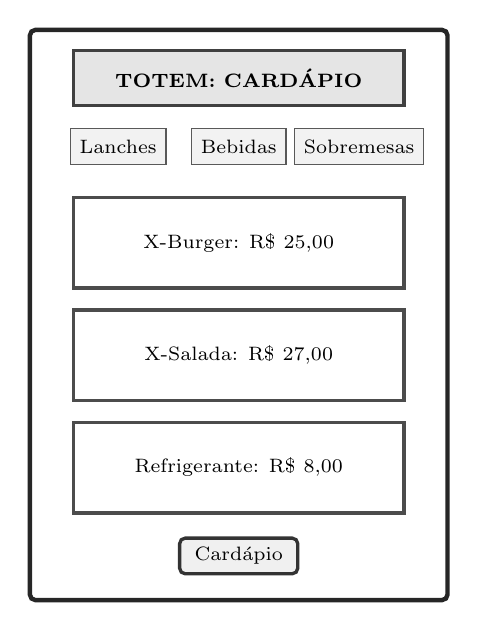
\begin{tikzpicture}[scale=1.02]
  \draw[moldura] (0,0) rectangle (5.2,7.1);
  \node[cabecalho] at (2.6,6.5) {TOTEM: CARDÁPIO};
  \node[categoria] at (1.1,5.65) {Lanches};
  \node[categoria] at (2.6,5.65) {Bebidas};
  \node[categoria] at (4.1,5.65) {Sobremesas};
  \node[cartao] at (2.6,4.45) {X-Burger: R\$ 25,00};
  \node[cartao] at (2.6,3.05) {X-Salada: R\$ 27,00};
  \node[cartao] at (2.6,1.65) {Refrigerante: R\$ 8,00};
  \node[botao] at (2.6,0.55) {Cardápio};
\end{tikzpicture}
\caption{Protótipo de baixa fidelidade: versão inicial elaborada em aula (reconstrução digital).}
\label{fig:wf_inicial}
\end{figure}

\section{Versão Completa (digital)}

A Figura~\ref{fig:wf_completa} apresenta a versão completa, com três telas interligadas: cardápio (US01), carrinho (US02) e personalização (US03). O botão ``Preciso de Ajuda'' aparece em todas as telas, antecipando a US07, embora esta não faça parte da Sprint 1.

\textbf{Acesso ao protótipo:} versão completa disponível no Figma, em \url{https://www.figma.com/make/K5XkfIlE4NsOd0QDdhzcSx/Restaurant-Kiosk-App-Design?t=oOAOxDcetEklvcdI-20&fullscreen=1}. A Figura~\ref{fig:wf_completa} é uma representação estática; o modelo dinâmico e navegável está no link indicado.

\begin{figure}[ht]
\centering
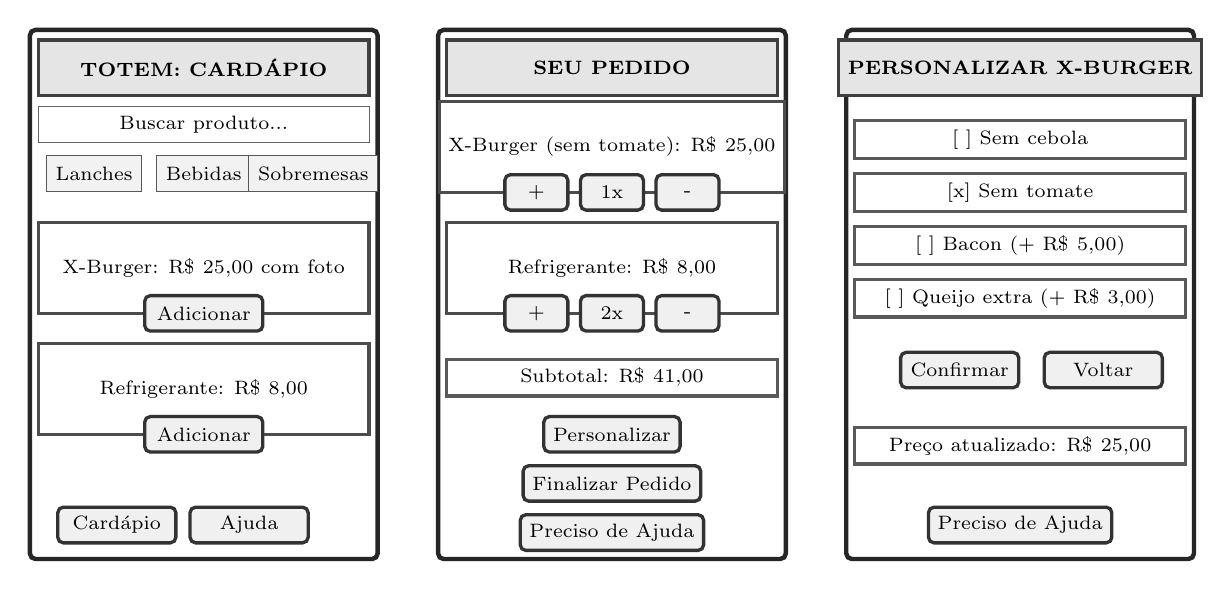
\begin{tikzpicture}[scale=0.96]
  % Tela 1: Cardápio
  \begin{scope}[xshift=0cm]
    \draw[moldura] (0,0) rectangle (4.6,7);
    \node[cabecalho] at (2.3,6.5) {TOTEM: CARDÁPIO};
    \node[campo] at (2.3,5.75) {Buscar produto...};
    \node[categoria] at (0.85,5.1) {Lanches};
    \node[categoria] at (2.3,5.1) {Bebidas};
    \node[categoria] at (3.75,5.1) {Sobremesas};
    \node[cartao] at (2.3,3.85) {X-Burger: R\$ 25,00 com foto};
    \node[botao] at (2.3,3.25) {Adicionar};
    \node[cartao] at (2.3,2.25) {Refrigerante: R\$ 8,00};
    \node[botao] at (2.3,1.65) {Adicionar};
    \node[botao] at (1.15,0.45) {Cardápio};
    \node[botao] at (2.9,0.45) {Ajuda};
  \end{scope}
  % Tela 2: Carrinho
  \begin{scope}[xshift=5.4cm]
    \draw[moldura] (0,0) rectangle (4.6,7);
    \node[cabecalho] at (2.3,6.5) {SEU PEDIDO};
    \node[cartao] at (2.3,5.45) {X-Burger (sem tomate): R\$ 25,00};
    \node[botaq] at (1.3,4.85) {+};
    \node[botaq] at (2.3,4.85) {1x};
    \node[botaq] at (3.3,4.85) {-};
    \node[cartao] at (2.3,3.85) {Refrigerante: R\$ 8,00};
    \node[botaq] at (1.3,3.25) {+};
    \node[botaq] at (2.3,3.25) {2x};
    \node[botaq] at (3.3,3.25) {-};
    \node[opcao] at (2.3,2.4) {Subtotal: R\$ 41,00};
    \node[botao] at (2.3,1.65) {Personalizar};
    \node[botao] at (2.3,1.0) {Finalizar Pedido};
    \node[botao] at (2.3,0.35) {Preciso de Ajuda};
  \end{scope}
  % Tela 3: Personalização
  \begin{scope}[xshift=10.8cm]
    \draw[moldura] (0,0) rectangle (4.6,7);
    \node[cabecalho] at (2.3,6.5) {PERSONALIZAR X-BURGER};
    \node[opcao] at (2.3,5.55) {[ ] Sem cebola};
    \node[opcao] at (2.3,4.85) {[x] Sem tomate};
    \node[opcao] at (2.3,4.15) {[ ] Bacon (+ R\$ 5,00)};
    \node[opcao] at (2.3,3.45) {[ ] Queijo extra (+ R\$ 3,00)};
    \node[botao] at (1.5,2.5) {Confirmar};
    \node[botao] at (3.4,2.5) {Voltar};
    \node[opcao] at (2.3,1.5) {Preço atualizado: R\$ 25,00};
    \node[botao] at (2.3,0.45) {Preciso de Ajuda};
  \end{scope}
\end{tikzpicture}
\caption{Protótipo de baixa fidelidade: versão completa: cardápio, carrinho e personalização.}
\label{fig:wf_completa}
\end{figure}

\section{Cobertura das User Stories}

\begin{table}[ht]
\centering
\caption{Relação entre as histórias da Sprint 1 e os elementos do protótipo.}
\resizebox{\textwidth}{!}{%
\begin{tabular}{@{}p{2.6cm}p{6cm}p{5cm}@{}}
\toprule
\textbf{História} & \textbf{Elemento no protótipo} & \textbf{Critério de aceitação atendido} \\
\midrule
US01 & Cabeçalho, categorias, cartões com foto e preço & Ao selecionar ``Cardápio'', exibir produtos por categoria com preços e fotos \\
US02 & Botão ``Adicionar'', carrinho com quantidade $+$ / $-$ & Ao clicar em ``Adicionar'', o item vai ao carrinho e permite aumentar a quantidade \\
US03 & Tela ``Personalizar'' com remoção de ingredientes e extras & Ao acessar item customizável, exibir opções como ``sem cebola'' ou ``bacon'' \\
\bottomrule
\end{tabular}%
}
\end{table}

\chapter{Diagramas de Caso de Uso}

\section{Versão Inicial (aula)}

A versão inicial foi esboçada em aula com o ator principal e os três casos de uso da Sprint 1, sem relacionamentos ou detalhamento de fluxo (Figura~\ref{fig:uc_inicial}).

\begin{figure}[ht]
\centering
\begin{tikzpicture}[scale=0.95]
  \node[inner sep=0pt] (ator) at (0,0) {%
    \begin{tikzpicture}[scale=0.55]
      \draw (0,0.9) circle (0.3);
      \draw (0,0.6) -- (0,-0.3);
      \draw (-0.45,0.25) -- (0.45,0.25);
      \draw (0,-0.3) -- (-0.45,-1.1);
      \draw (0,-0.3) -- (0.45,-1.1);
    \end{tikzpicture}
  };
  \node[below=0.1cm of ator] {Cliente};
  \node[draw, ellipse, minimum width=4.6cm, minimum height=1cm] (uc1) at (5,2) {UC01: Visualizar Cardápio};
  \node[draw, ellipse, minimum width=4.6cm, minimum height=1cm] (uc2) at (5,0) {UC02: Adicionar Item};
  \node[draw, ellipse, minimum width=4.6cm, minimum height=1cm] (uc3) at (5,-2) {UC03: Personalizar Pedido};
  \draw (ator.east) -- (uc1.west);
  \draw (ator.east) -- (uc2.west);
  \draw (ator.east) -- (uc3.west);
\end{tikzpicture}
\caption{Diagrama de caso de uso: versão inicial elaborada em aula (reconstrução digital).}
\label{fig:uc_inicial}
\end{figure}

\section{Versão Completa (digital)}

A versão completa (Figura~\ref{fig:uc_completa}) acrescenta a fronteira do sistema, os relacionamentos de inclusão e extensão e a especificação sumária de cada caso de uso. O código-fonte em formato digital está no arquivo \texttt{caso\_uso\_sprint1.puml}, na pasta \texttt{diagramas}, mantido junto ao projeto. A versão editável em ferramenta de diagramação está disponível no Lucidchart: \url{https://lucid.app/lucidchart/87d422f6-cbc5-4222-96b6-cc3525e06341/edit?invitationId=inv_f1629cb9-e852-4390-acda-172a5c572f27&page=0_0#}.

\begin{figure}[ht]
\centering
\begin{tikzpicture}[scale=0.9]
  \node[inner sep=0pt] (ator) at (-0.6,0) {%
    \begin{tikzpicture}[scale=0.55]
      \draw (0,0.9) circle (0.3);
      \draw (0,0.6) -- (0,-0.3);
      \draw (-0.45,0.25) -- (0.45,0.25);
      \draw (0,-0.3) -- (-0.45,-1.1);
      \draw (0,-0.3) -- (0.45,-1.1);
    \end{tikzpicture}
  };
  \node[below=0.1cm of ator] {Cliente};
  \node[draw, ellipse, minimum width=5cm, minimum height=1.05cm] (uc1) at (5.3,2.1) {UC01: Visualizar Cardápio};
  \node[draw, ellipse, minimum width=5cm, minimum height=1.05cm] (uc2) at (5.3,0) {UC02: Adicionar Item ao Carrinho};
  \node[draw, ellipse, minimum width=5cm, minimum height=1.05cm] (uc3) at (5.3,-2.1) {UC03: Personalizar Pedido};
  \node[draw, dashed, rounded corners, fit=(uc1)(uc2)(uc3), inner sep=0.7cm,
        label={[anchor=south, font=\scriptsize\bfseries]above:Sistema Totem de Autoatendimento}] (sistema) {};
  \draw (ator.east) -- (uc1.west);
  \draw (ator.east) -- (uc2.west);
  \draw (ator.east) -- (uc3.west);
  \draw[->] (uc2.east) -- node[above, sloped, font=\scriptsize] {$\langle\langle$include$\rangle\rangle$} (uc1.east);
  \draw[->] (uc3.east) -- node[below, sloped, font=\scriptsize] {$\langle\langle$extend$\rangle\rangle$} (uc2.east);
\end{tikzpicture}
\caption{Diagrama de caso de uso: versão completa: fronteira do sistema e relacionamentos.}
\label{fig:uc_completa}
\end{figure}

\section{Especificação dos Casos de Uso}

\begin{table}[ht]
\centering
\caption{Especificação sumária dos casos de uso da Sprint 1.}
\resizebox{\textwidth}{!}{%
\begin{tabular}{@{}p{2.3cm}p{3.4cm}p{4.2cm}p{4.2cm}@{}}
\toprule
\textbf{UC} & \textbf{Ator} & \textbf{Fluxo principal} & \textbf{Pós-condição} \\
\midrule
UC01 & Cliente & Acessa o totem, seleciona ``Cardápio'', navega entre categorias & Produtos exibidos com categorias, preços e fotos \\
UC02 & Cliente & Seleciona produto, clica em ``Adicionar'', ajusta quantidade & Item presente no carrinho com quantidade definida \\
UC03 & Cliente & Acessa item customizável, remove ingrediente ou adiciona extra & Pedido personalizado com preço recalculado \\
\bottomrule
\end{tabular}%
}
\end{table}

\chapter{Captura de Feedback do Protótipo}

\section{Instrumento de Coleta}

Foram definidas três tarefas, uma por história da Sprint 1, todas executadas sobre a versão completa do protótipo (Figura~\ref{fig:wf_completa}):

\begin{enumerate}
  \item \textbf{Tarefa 1 (US01):} localizar a categoria ``Lanches'', encontrar o X-Burger e conferir foto e preço.
  \item \textbf{Tarefa 2 (US02):} adicionar um X-Burger e dois refrigerantes ao carrinho e aumentar a quantidade do refrigerante.
  \item \textbf{Tarefa 3 (US03):} personalizar o X-Burger removendo o tomate e adicionando bacon.
\end{enumerate}

Após as tarefas, o participante respondeu a três perguntas: (i) conseguiu concluir sem ajuda?; (ii) em qual etapa teve maior dificuldade?; (iii) que mudança sugere antes da implementação? As respostas são anônimas e o instrumento não coleta dados pessoais, em continuidade ao TCLE da Parcial 1.

\section{Matriz de Captura de Feedback}

A matriz da Tabela~\ref{tab:matriz_feedback} cruza as dimensões observadas com os participantes, obtidos no teste do protótipo.

\begin{table}[ht]
\centering
\caption{Matriz de captura de feedback do protótipo de baixa fidelidade.}
\label{tab:matriz_feedback}
\resizebox{\textwidth}{!}{%
\begin{tabular}{@{}p{3.6cm}p{2.6cm}p{2.6cm}p{2.6cm}p{2.6cm}@{}}
\toprule
\textbf{Dimensão} & \textbf{P1} & \textbf{P2} & \textbf{P3} & \textbf{P4} \\
\midrule
Concluiu Tarefa 1 (US01) & Sim & Sim & Sim & Sim \\
Concluiu Tarefa 2 (US02) & Sim & Sim & Sim & Não \\
Concluiu Tarefa 3 (US03) & Sim & Não & Sim & Sim \\
Precisou de ajuda? & Não & Sim & Não & Sim \\
Clareza das categorias & Sim & Sim & Sim & Sim \\
Clareza do carrinho & Sim & Não & Sim & Não \\
Clareza da personalização & Sim & Não & Sim & Sim \\
Acessibilidade / tamanho da fonte & Não & Não & Sim & Não \\
Sugestão principal & Rapidez e fotos & Ajuda para personalizar & Modo fácil & PIX e senha \\
\bottomrule
\end{tabular}%
}
\end{table}

\section{Dados Coletados}

\begin{table}[ht]
\centering
\caption{Registro individual dos participantes do teste de usabilidade.}
\resizebox{\textwidth}{!}{%
\begin{tabular}{@{}p{1.7cm}p{2.6cm}p{2.6cm}p{2.6cm}p{2.6cm}p{2.4cm}@{}}
\toprule
\textbf{Part.} & \textbf{Tarefas concluídas} & \textbf{Tempo total} & \textbf{Ajuda necessária} & \textbf{Satisfação (1 a 5)} & \textbf{Sugestão} \\
\midrule
P1 & 3/3 & 184 s & Não & 5 & Rapidez e fotos \\
P2 & 2/3 & 246 s & Sim & 4 & Ajuda para personalizar \\
P3 & 3/3 & 205 s & Não & 5 & Modo fácil \\
P4 & 2/3 & 278 s & Sim & 3 & PIX e senha \\
\bottomrule
\end{tabular}%
}
\end{table}

A síntese dos dados aponta a acessibilidade e a ajuda na personalização e a acessibilidade entre as principais sugestões, encaminhando ajustes ao \textit{Product Backlog} e ao próximo \textit{Sprint Backlog}.

\chapter{Sprint Review e Retrospectiva}

\section{Sprint Review}

A Sprint Review foi conduzida com a demonstração das US01 e US02; a US03 teve o protótipo validado, mas a implementação não foi concluída e retornou ao \textit{Product Backlog}. O roteiro seguiu a coluna ``Como Demonstrar'' do \textit{Product Backlog} da Parcial 1 (Tabela~\ref{tab:demo}).

\begin{table}[ht]
\centering
\caption{Roteiro de demonstração usado na Sprint Review.}
\label{tab:demo}
\resizebox{\textwidth}{!}{%
\begin{tabular}{@{}p{1.2cm}p{4cm}p{8.5cm}@{}}
\toprule
\textbf{ID} & \textbf{Funcionalidade} & \textbf{Como demonstrar} \\
\midrule
01 & Visualizar Cardápio com Fotos & Abrir o totem, ver a tela inicial e navegar entre as categorias \\
02 & Adicionar ao Carrinho & Selecionar um hambúrguer e adicionar 2 refrigerantes \\
03 & Personalização de Itens & Selecionar ``X-Burger'' e remover o tomate \\
\bottomrule
\end{tabular}%
}
\end{table}

\textbf{Data e participantes:} 26/10/2026, Gabriel Muzel e Mateus Iuri. \textbf{Feedback recebido:} US01 e US02 demonstradas com sucesso; US03 não foi concluída e retornou ao backlog. \textbf{Decisões tomadas:} manter a acessibilidade como prioridade e registrar o destino das histórias no quadro Kanban.

\section{Retrospectiva}

\begin{itemize}
  \item \textbf{Data e participantes:} 26/10/2026, Gabriel Muzel e Mateus Iuri.
  \item \textbf{O que funcionou bem:} execução do roteiro de demonstração e preenchimento da matriz de feedback com os participantes.
  \item \textbf{O que pode melhorar:} dependência de imagens do Figma e conclusão da US03, que voltou ao \textit{Product Backlog}.
  \item \textbf{Ações de melhoria combinadas e responsáveis:} Gabriel fica responsável por registrar o link dinâmico do protótipo e Mateus por reestimar a US03 na próxima sprint.
\end{itemize}

\section{Alterações no Product Backlog (antes e depois)}
\label{sec:backlog}

A coluna ``Antes'' reproduz o \textit{Product Backlog} registrado na Parcial 1. A coluna ``Depois'' registra o resultado da Sprint Review; quando não houve revisão explícita, mantém-se a configuração anterior.

\begin{table}[ht]
\centering
\caption{Product Backlog: antes e depois da Sprint Review.}
\resizebox{\textwidth}{!}{%
\begin{tabular}{@{}cp{4.6cm}cp{2.2cm}c@{}}
\toprule
\textbf{ID} & \textbf{Funcionalidade} & \textbf{Imp. antes} & \textbf{PH antes} & \textbf{Depois da Sprint 1 (Imp./PH)} \\
\midrule
01 & Visualizar Cardápio com Fotos & 30 & 5 & sem alteração \\
02 & Adicionar ao Carrinho & 30 & 3 & sem alteração \\
03 & Personalização de Itens & 30 & 8 & 30/8, mantida no backlog \\
04 & Pagamento Integrado (PIX/Cartão) & 30 & 13 & sem alteração \\
05 & Tela de Sucesso e Senha & 25 & 3 & sem alteração \\
06 & Painel de Acompanhamento (Admin) & 30 & 8 & sem alteração \\
07 & Acessibilidade (Modo Fácil) & 25 & 5 & sem alteração \\
08 & Botão de Ajuda / Suporte & 20 & 3 & sem alteração \\
09 & Cadastro de Produtos (Admin) & 20 & 5 & sem alteração \\
10 & Edição/Exclusão de Produtos (Admin) & 15 & 3 & sem alteração \\
11 & Modo de Espera (Atração) & 5 & 2 & sem alteração \\
12 & Relatório de Vendas Diárias (Admin) & 15 & 5 & sem alteração \\
\bottomrule
\end{tabular}%
}
\end{table}

\section{Alterações no Quadro Kanban (antes e depois)}

O quadro foi gerenciado no Trello, cujo convite está disponível em \url{https://trello.com/invite/b/6ad94663283aa9fb3397a1d4/ATTI75eb7223eddb3d284cc9695b8728757a2B864393/kanban}. As Figuras~\ref{fig:kanban_antes} e \ref{fig:kanban_depois} registram o estado do quadro antes e depois da Sprint 1. Na primeira imagem, as colunas eram \textit{Product Backlog} (US04), \textit{Sprint Backlog} (US01, US02 e US03) e \textit{Done} vazia. Na segunda, US01 e US02 foram para \textit{Done}; US03 retornou para \textit{Product Backlog} por não ter sido concluída; US04 permaneceu no \textit{Product Backlog}; e a coluna \textit{Sprint Backlog} ficou vazia.

\begin{figure}[ht]
\centering
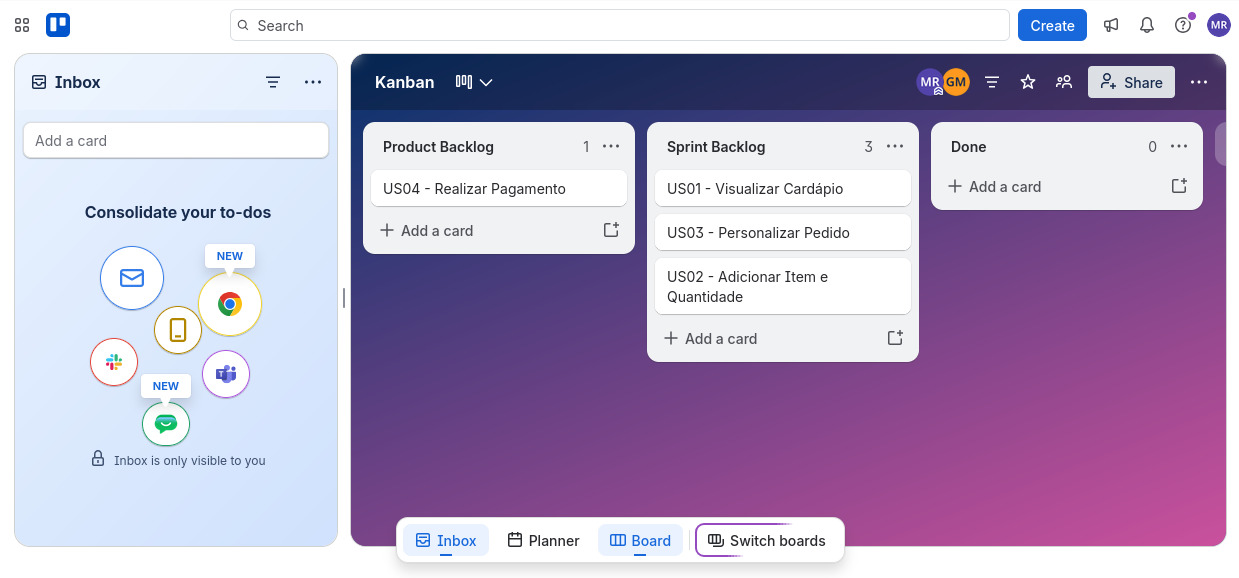
\includegraphics[width=\textwidth]{../documentos/kanban1.jpeg}
\caption{Quadro Kanban antes da Sprint 1: US01, US02 e US03 no Sprint Backlog; Done vazia.}
\label{fig:kanban_antes}
\end{figure}

\begin{figure}[ht]
\centering
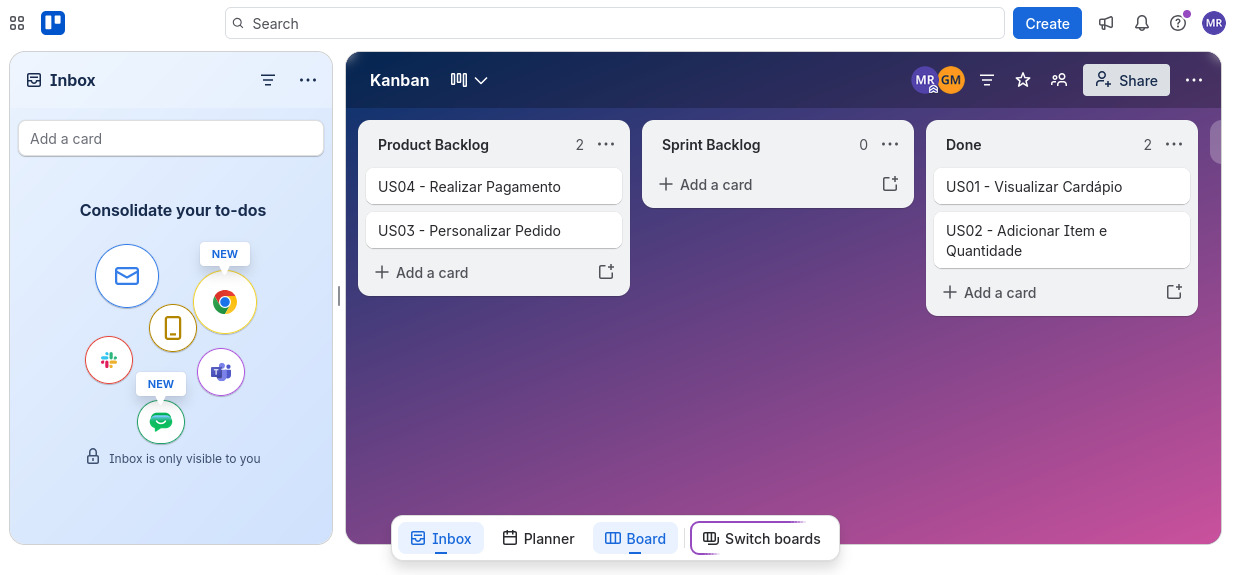
\includegraphics[width=\textwidth]{../documentos/kanban2.jpeg}
\caption{Quadro Kanban depois da Sprint 1: US01 e US02 em Done; US03 de volta ao Product Backlog.}
\label{fig:kanban_depois}
\end{figure}

A Tabela~\ref{tab:kanban_us} resume a movimentação por história, observada diretamente nas imagens.

\begin{table}[ht]
\centering
\caption{Movimentação das histórias no quadro Kanban.}
\label{tab:kanban_us}
\resizebox{\textwidth}{!}{%
\begin{tabular}{@{}p{5cm}p{4cm}p{5cm}@{}}
\toprule
\textbf{História} & \textbf{Antes} & \textbf{Depois} \\
\midrule
US01: Visualizar Cardápio & Sprint Backlog & Done \\
US02: Adicionar Item e Quantidade & Sprint Backlog & Done \\
US03: Personalizar Pedido & Sprint Backlog & Product Backlog (não concluída) \\
US04: Realizar Pagamento & Product Backlog & Product Backlog (permanece) \\
Coluna Sprint Backlog & 3 cartões & vazia \\
Coluna Done & vazia & 2 cartões \\
\bottomrule
\end{tabular}%
}
\end{table}

A Tabela~\ref{tab:kanban} mantém o detalhamento das tarefas técnicas registrado no \textit{Sprint Backlog} da Parcial 1. A coluna ``Depois (história)'' informa o destino da história correspondente, visível nas imagens; o status individual de cada tarefa técnica não pode ser inferido das capturas de tela.

\begin{table}[ht]
\centering
\caption{Detalhamento das tarefas da Sprint 1 e destino de cada história.}
\label{tab:kanban}
\resizebox{\textwidth}{!}{%
\begin{tabular}{@{}p{3cm}p{5.8cm}c@{}p{4cm}}
\toprule
\textbf{História} & \textbf{Tarefa técnica} & \textbf{Resp.} & \textbf{Depois (história)} \\
\midrule
US01 & Protótipo de baixa fidelidade no Figma (versão completa) & Gabriel & Done \\
US01 & Estrutura HTML/CSS da tela de cardápio & Mateus & Done \\
US01 & Integrar com API/JSON de produtos & Mateus & Done \\
US02 & Estado global do carrinho (Context) & Gabriel & Done \\
US02 & Componente botão ``Adicionar'' & Gabriel & Done \\
US02 & Drawer lateral do carrinho & Mateus & Done \\
US03 & Tela modal de opções de ingredientes & Mateus & Product Backlog \\
US03 & Lógica de subtração/acréscimo de preços & Gabriel & Product Backlog \\
US03 & Testar fluxo de item personalizado & Gabriel & Product Backlog \\
\bottomrule
\end{tabular}%
}
\end{table}

\chapter{Links de Acesso e Versionamento}

\begin{table}[ht]
\centering
\caption{Artefatos do projeto e respectivos links.}
\resizebox{\textwidth}{!}{%
\begin{tabular}{@{}p{4.2cm}p{10cm}@{}}
\toprule
\textbf{Artefato} & \textbf{Local / link} \\
\midrule
Quadro Kanban (Trello) & \url{https://trello.com/invite/b/6ad94663283aa9fb3397a1d4/ATTI75eb7223eddb3d284cc9695b8728757a2B864393/kanban} \\
Repositório Git & https://github.com/Fatec-activities-cb/eng-de-software.git \\
Protótipo no Figma & \href{https://www.figma.com/make/K5XkfIlE4NsOd0QDdhzcSx/Restaurant-Kiosk-App-Design?t=oOAOxDcetEklvcdI-20\&fullscreen=1}{Figma (protótipo)} \\
Diagrama de caso de uso (Lucidchart) & \href{https://lucid.app/lucidchart/87d422f6-cbc5-4222-96b6-cc3525e06341/edit?invitationId=inv_f1629cb9-e852-4390-acda-172a5c572f27\&page=0_0\#}{Lucidchart (diagrama editável)} \\
Diagrama de caso de uso (código) & arquivo local \texttt{../documentos/diagramas/caso\_uso\_sprint1.puml} \\
Quadro Kanban (imagens) & arquivos locais \texttt{../documentos/kanban1.jpeg} (antes) e \texttt{../documentos/kanban2.jpeg} (depois) \\
Relatório da Parcial 1 & arquivo local \texttt{parcial1.tex} \\
Relatório da Parcial 2 & arquivo local \texttt{parcial2.tex} \\
Dados do formulário & arquivo local \texttt{../documentos/formulario\_andromeda.csv} \\
Versionamento & repositório GitHub: \url{https://github.com/Fatec-activities-cb/eng-de-software.git} \\
\bottomrule
\end{tabular}%
}
\end{table}

Todo o versionamento é feito no repositório GitHub, já publicado. Os links foram validados em 26/10/2026.

\chapter{Considerações Finais}

A Parcial 2 registra os artefatos de projeto da Sprint 1 (protótipo de baixa fidelidade e diagramas de caso de uso), a captura de feedback e os eventos de encerramento da sprint. As decisões da Review e da Retrospectiva e o destino das histórias no quadro Kanban encontram-se registrados nas seções correspondentes.

% ---------------------------------
% ELEMENTOS PÓS-TEXTUAIS
% ---------------------------------
\phantompart
\postextual

% ---------------------------------
% Referências bibliográficas
% ---------------------------------
\bibliography{../documentos/references}

% ---------------------------------
% Glossário
% ---------------------------------

% ---------------------------------
% Apêndices
% ---------------------------------
\begin{apendicesenv}
\partapendices

\chapter{Diagrama de Caso de Uso da Aula}

\begin{figure}[!ht]
\setlength{\itemsep}{0pt}
\setlength{\parskip}{0pt}
\centering
\includegraphics[width=0.8\columnwidth]{imagens/diagrama_aula.png}
\caption{Diagrama de caso de uso produzido em aula.}
\end{figure}

\end{apendicesenv}

% ----------------------------------------------
% Anexos
% ----------------------------------------------
\begin{anexosenv}
\partanexos

\chapter{Quadro Kanban}

As Figuras~\ref{fig:kanban_antes} e \ref{fig:kanban_depois}, apresentadas no corpo deste relatório, registram o quadro antes e depois da Sprint 1. O quadro digital está disponível em \url{https://trello.com/invite/b/6ad94663283aa9fb3397a1d4/ATTI75eb7223eddb3d284cc9695b8728757a2B864393/kanban}.

\end{anexosenv}

%------------------------------------------------------
% INDICE REMISSIVO
%------------------------------------------------------
\phantompart
\printindex

\end{document}
